% Title: Report LaTex File: Concept Development
% Auther: DC Eksteen
% Student Number: 22623906
% Contact: 22623906@sun.ac.za
% Date: 2022/09/22
% Version: 2.0

\chapter{Concept Design and Evaluation}
% Section overview:

This section aims to identify and refine any requirements that were required of the training platform, and then demonstrate and analyse a concept solution that will be expanded into the final delivered demonstration model in further sections.

Table \ref{tab:conditions} shows the user requirements that were derived from the project objectives and literature review. These user requirements are then analysed in Section \ref{sec:req} to determine the performance and functional engineering requirements.

\begin{table}[H]
	%\renewcommand{\arraystretch}{\tablestretch}
	\centering
	\caption{Derived User Requirements}
	\begin{tabularx}{\textwidth}{>{\raggedright UR~}p{1.5 cm} X >{\raggedright\arraybackslash}p{2cm}}
		\toprule
		\multicolumn{2}{c}{User Requirement} & Priority                                                   \\
		\midrule
		\newR{UR:zwift}                      & Connect with Zwift                             & Essential \\
		\newR{UR:sim}                        & Realistic Riding Simulation                    & Essential \\
		\newR{UR:measure}                    & Accurate Measured Training Data                & Medium    \\
		\newR{UR:weight}                     & Weight Should be Comparable to Market Products & High      \\
		\newR{UR:range}                      & Accept a Wide Range of Bicycles                & High      \\
		\newR{UR:price}                      & Less Expensive than Market Products            & High      \\
		\newR{UR:store}                      & Platform Easily Stored                         & Medium    \\
		\bottomrule
	\end{tabularx}
	\label{tab:conditions}
\end{table}

\setcounter{reqCount}{0}

\newpage

\section{Requirement Analysis}
\label{sec:req}

\begin{table}[H]
	\renewcommand{\arraystretch}{\tablestretch}
	\centering
	\caption{Functional Engineering Requirements}
	\begin{tabularx}{\textwidth}{>{\raggedright FER~}p{0.8 cm} X >{\centering\arraybackslash}p{1.7cm}}
		\toprule
		\multicolumn{2}{c}{Functional Requirement} & Reference                                                                                 \\
		\midrule
		\newR{FR:ble}                              & Have \ac{ble} or ANT+ Connectivity                                  & UR \ref{UR:zwift}   \\
		\newR{FR:wheel}                            & \capitalisefmtwords{Accommodate both 27.5' and 29' wheel diameters} & UR \ref{UR:range}   \\
		\newR{FR:speed}                            & \capitalisefmtwords{Be Able to Determine Wheel Speed}               & UR \ref{UR:measure} \\
		\bottomrule
	\end{tabularx}
	\label{tab:funcreq}
\end{table}

\setcounter{reqCount}{0}

\begin{table}[H]
	\renewcommand{\arraystretch}{\tablestretch}
	\centering
	\caption{Performance Engineering Requirements}
	\begin{tabularx}{\textwidth}{>{\raggedright PER~}p{0.8 cm} X p{1.1cm} p{1.6cm} p{1cm} >{\centering\arraybackslash}p{1.7cm}}
		\toprule
		\multicolumn{2}{c}{Performance Requirement} & Target                  & Value & Unit     & Reference                                      \\
		\midrule
		\newR{PR:wheelbase}                         & Allowable Wheelbase     & Range & 900-1200 & \si{\milli\meter}         & UR~\ref{UR:range}  \\
		\newR{PR:weight}                            & Weight                  & Max   & 8        & \si{\kilogram}            & UR~\ref{UR:weight} \\
		\newR{PR:speed}                             & Simulated Moving Speed  & Max   & 60       & \si{\kilo\meter\per\hour} & UR~\ref{UR:sim}    \\
		\newR{PR:27speed}                           & Wheel Speed (27.5')     & Max   & 2900     & \ac{rpm}                  & UR \ref{UR:sim}    \\
		\newR{PR:29speed}                           & Wheel Speed (29')       & Max   & 3500     & \ac{rpm}                  & UR \ref{UR:sim}    \\
		\newR{PR:torque}                            & Torque Applied to Wheel & Min   & 12       & \si{\newton\meter}        & UR \ref{UR:sim}    \\
		\bottomrule
	\end{tabularx}
	\label{tab:perfreq}
\end{table}

\subsection{Operating Conditions}
\label{sec:opspeedc}

\subsubsection{PER \ref{PR:27speed} \& \ref{PR:29speed}:}

The typical speed of a cyclist typically ranges from \SI{10}{\kilo\meter\per\hour} to \SI{50}{\kilo\meter\per\hour} when cycling on reasonably flat ground. For the design of the platform, a speed of maximum required speed of \SI{60}{\kilo\meter\per\hour} was assumed. Considering the two wheel sizes that were identified in Section~\ref{sec:specs}, the expected wheel rotational speeds are determined by Equation~\ref{eq:omega}.

\begin{equation}
	\ac{omega} = \frac{2 \ac{v}}{D_{wheel}}
	\label{eq:omega}
\end{equation}

\subsubsection{PER \ref{PR:torque}:}

Typically, amateur cyclists maintain an average power output between \SI{75}{\watt} and \SI{100}{\watt}, and pro cyclists can maintain up to \SI{400}{\watt}, during a 1 hour workout. As the cyclist's speed increases, less torque is required to maintain the same power output. The relation is expressed as Equation~\ref{eq:pow} and can be used to determine the torque that would need to be applied at different wheel speeds to achieve these power outputs.

\section{Concept Design}
\label{sec:conc}

A general overview of the concept starts by distinguishing what falls within the \acf{nsoi}, \acf{wsoi} and the outside environment. Elements in the \ac{wsoi} are not part of the scope of the concept, yet interact directly with the proposed system during normal operation. Elements in the outside Environment may have an influence on the system, but will not be affected by the platform during normal operation. Figure~\ref{fig:soi} shows the boundaries between the \ac{nsoi}, \ac{wsoi} and Environment for the concept that was developed.

\begin{figure}[H]
	\begin{center}
		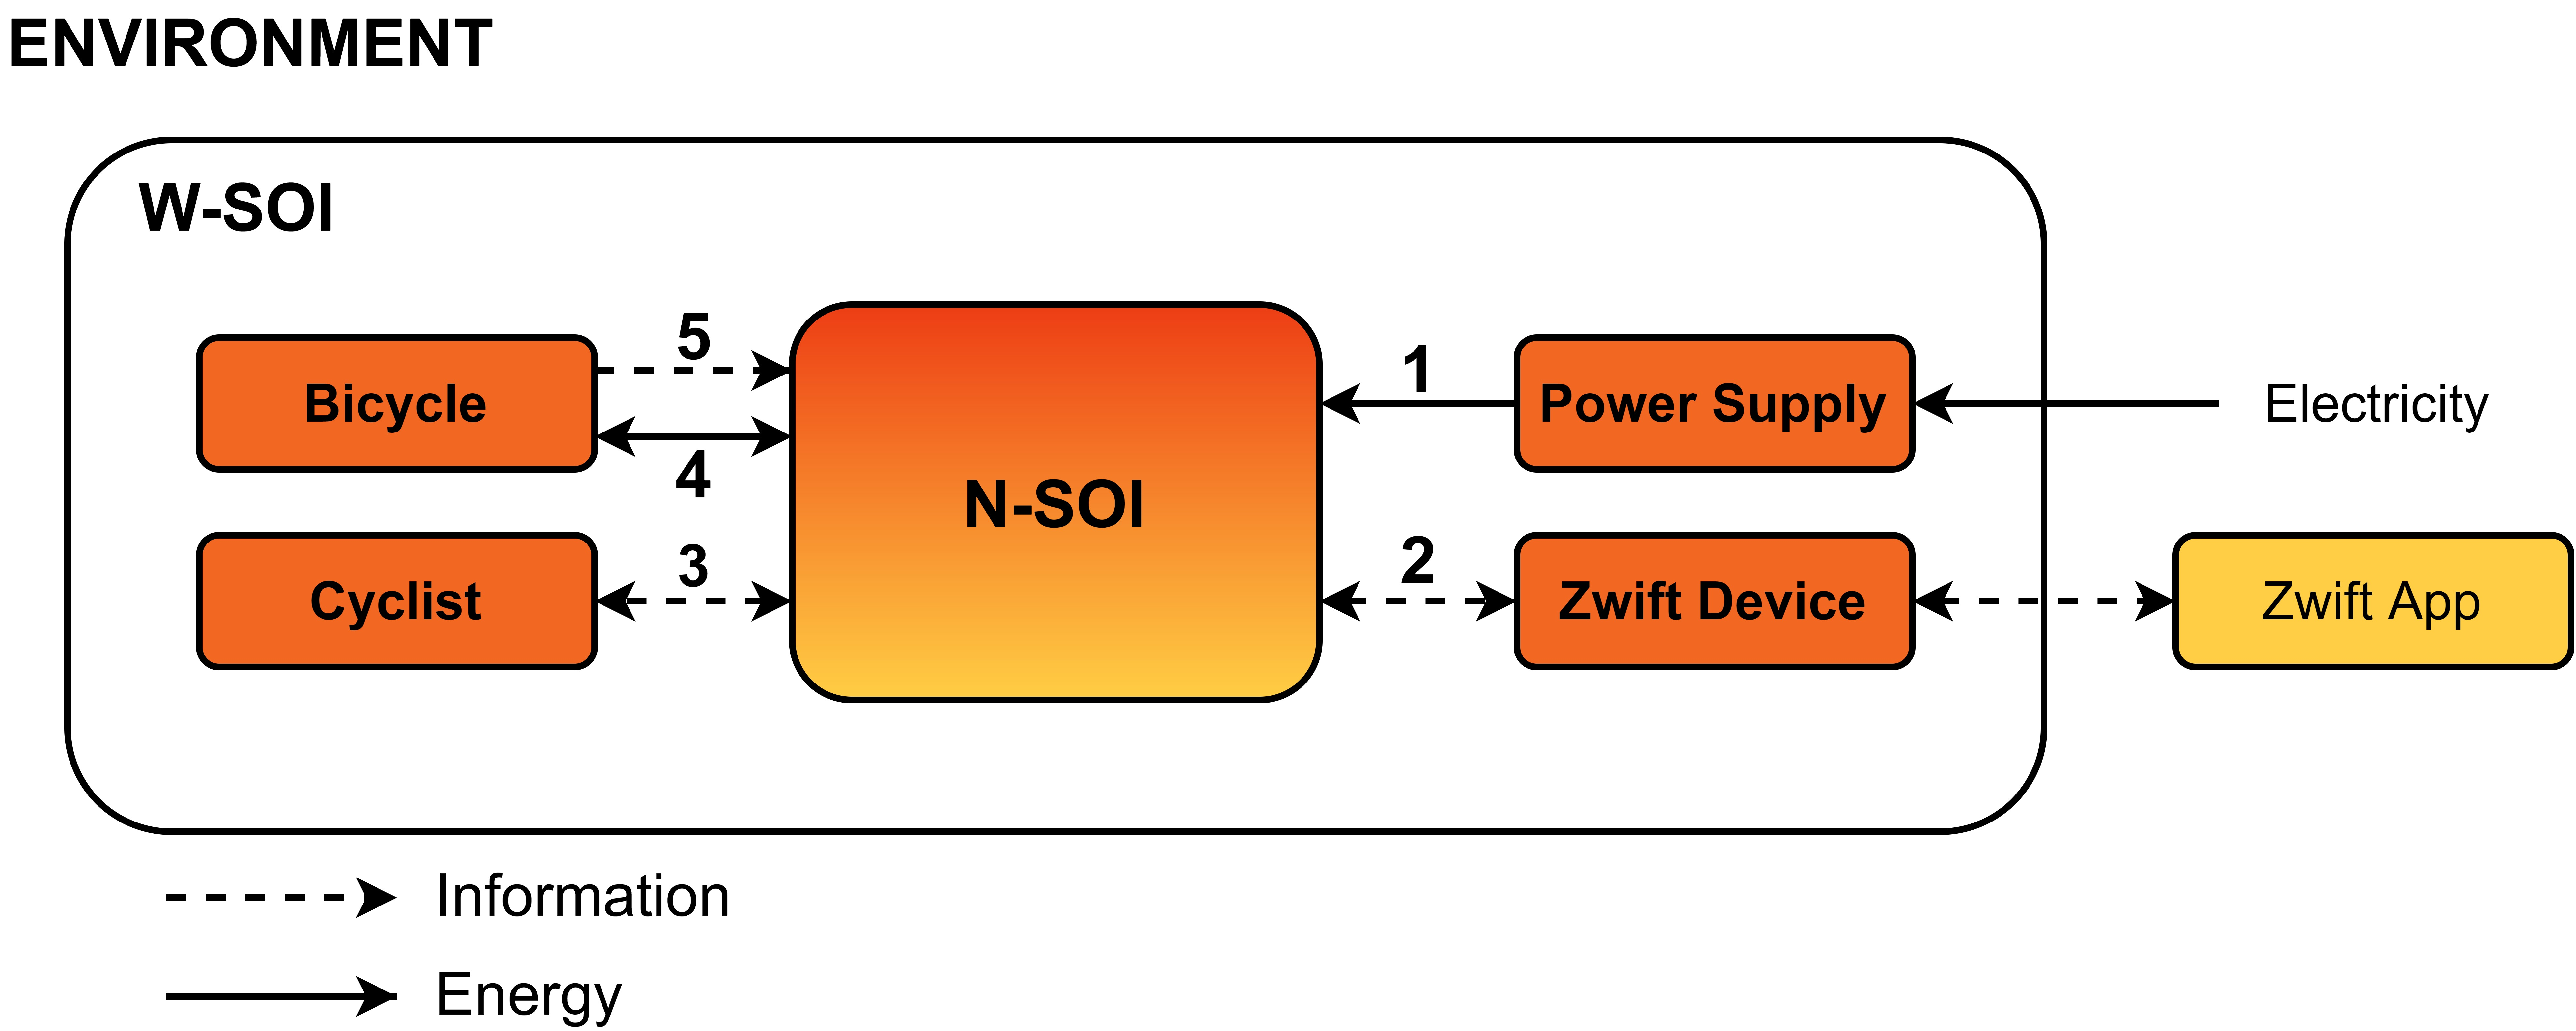
\includegraphics[width=\textwidth]{SOI.jpg}
		\caption{Concept Boundary of Interest}
		\label{fig:soi}
	\end{center}
\end{figure}

The interfaces between elements are explained in Table~\ref{tab:links}.

\begin{table}[H]
	\renewcommand{\arraystretch}{\tablestretch}
	\centering
	\caption{Concept Boundary Interfaces}
	\begin{tabularx}{\textwidth}{p{1.5cm} X p{4cm}}
		\toprule
		Interface & Description                                           & Type               \\
		\midrule
		1         & \capitalisefmtwords{Power delivery to platform}       & Electrical Energy  \\
		2         & \ac{ble} with \ac{ftms} implementation                & Communication Info \\
		3         & \capitalisefmtwords{User inputs and feedback to user} & User Info          \\
		4         & \capitalisefmtwords{Resistance applied to bicycle}    & Energy Losses      \\
		5         & \capitalisefmtwords{Sensor readings of cycling data}  & Sensor Info        \\
		\bottomrule
	\end{tabularx}
	\label{tab:links}
\end{table}

\subsubsection{2:}
It was decided to keep the platform completely separate from the device that will be running the Zwift application, as this will allow th platform to easily be used by any other device without requiring any additional modifications.\ac{ble} was chosen as the communication protocol as this is what is available on most consumer electronic devices that Zwift is expected to operate on, and will thus not need an external unit to communicate with the platform.

\section{Concept Evaluation}
\label{sec:eval}

\begin{table}[H]
	\renewcommand{\arraystretch}{\tablestretch}
	\centering
	\caption{Concept Requirement Fulfilment Analysis}
	\begin{tabularx}{\textwidth}{p{1.5cm} X p{4cm}}
		\toprule
		Requirement & Proposed Solution                                     & Level of Success   \\
		\midrule
		1           & \capitalisefmtwords{Power delivery to platform}       & Pass  \\
		2           & \ac{ble} with \ac{ftms} implementation                & Pass \\
		3           & \capitalisefmtwords{User inputs and feedback to user} & Pass \\
		4           & \capitalisefmtwords{Resistance applied to bicycle}    & Pass \\
		5           & \capitalisefmtwords{Sensor readings of cycling data}  & Pass \\
		\bottomrule
	\end{tabularx}
	\label{tab:eval}
\end{table}